
\section{Algoritmi}
\label{cap:algorithms}

\subsection{MST2Approximation}

MST2Approximation è l'implementazione dell'algoritmo di $2$-approssimazione basato sul Minimum Spanning Tree visto a lezione. L'algoritmo prevede i seguenti step:

\begin{enumerate}
    \item Selezionare un vertice radice $root$ arbitrario;
    \item Ricavare l'MST del grafo in input a partire da $root$, utilizzando ad esempio l'algoritmo di Prim;
    \item Eseguire una visita pre-order dell'MST ricavato al passo precedente;
    \item Aggiungere la radice $root$ pre-order alla fine della lista ritornata dalla visita pre-order.
    \item Calcolare il peso totale del circuito ricavato nei 2 passi precedenti e restituire il risultato.
\end{enumerate}

\noindent Il listato \ref{listing:tsp2approx} contiene la nostra implementazione dell'algoritmo, step per step.\\

\begin{listing}[!ht]
\begin{minted}{c++}
// MST2Approximation/approx_tsp.h

// Step 1
random_generator::IntegerRandomGenerator random(0, distance_matrix.size() - 1);
const size_t root = random();

// Step 2
std::vector<Edge> mst(mst::prim_binary_heap_mst(distance_matrix, root));

// Step 3, 4
DFS dfs(std::move(mst));
const auto circuit = dfs.preorder_traversal();

// Funzione lambda che calcola la distanza tra due vertici
const auto get_distance = [&distance_matrix](const size_t x, const size_t y) {
    return distance_matrix.at(x, y);
};

// Step 5
return utils::sum_weights_in_circuit(circuit.cbegin(), circuit.cend(), get_distance);
\end{minted}
\caption{Implementazione di TSP 2-approssimato. I commenti del file originale sono stati omessi per una maggiore compattezza.}
\label{listing:tsp2approx}
\end{listing}

\noindent L'algoritmo TSP 2-approssimato è stato implementato a partire dallo pseudo codice visto in classe. \\

\subsubsection{Osservazioni}

\begin{itemize}
    \item Abbiamo usato l'algoritmo di Prim per eseguire il calcolo del Minimum Spanning Tree. Esso è infatti più adatto rispetto a Kruskal quando il grafo è rappresentato come Matrice della Distanze. Kruskal richiede di estrarre la lista di lati ordinata in modo ascendente rispetto al peso all'inizio dell'algoritmo, mentre Prim necessita solo della lista dei vertici. Ricordiamo che in un grafo completo vale l'equivalenza \complexityCompleteGraph{}.

    \item La coda di priorità usata dall'algoritmo di Prim è stata implementata con una Min Heap binaria, la quale è già stata descritta in dettaglio nella relazione del primo progetto.

    \item Come notato nella sezione \hyperref[alternative-graph-representation]{Rappresentazione alternativa del grafo: caso MST}, l'albero di copertura minimo è rappresentato come Mappa di Adiacenza all'interno di \codeinline{Shared/DFS.h}.

    \item Il metodo \mintinline{c++}{DFS::preorder_traversal} invoca al suo interno il metodo ricorsivo \\
    \mintinline{c++}{DFS::preorder_traversal_rec}. Il listato \ref{listing:dfs} contiene la definizione di tale metodo.
\end{itemize}

\begin{listing}[!ht]
\begin{minted}{c++}
// Shared/DFS.h

void preorder_traversal_rec(size_t v, std::unordered_set<size_t>& visited,
                            std::vector<size_t>& circuit) const {
  visited.insert(v);
  circuit.push_back(v);

  for (const auto& [u, _] : adjacency_map.adjacent_vertexes(v)) {
    // se un nodo adiacente non è stato visitato, viene visitato
    // ricorsivamente
    if (!visited.count(u)) {
      preorder_traversal_rec(u, visited, circuit);
    }
  }
}
\end{minted}
\caption{Implementazione ricorsiva della visita pre-order, inizialmente invocata sul nodo $0$. I commenti del file originale sono stati omessi per una maggiore compattezza.}
\label{listing:dfs}
\end{listing}

\subsection{HeldKarp}

Riportiamo lo pseudocodice dell'algortimo di programmazione dinamica Held \& Karp. La funzione \codeinline{HeldKarp(S, v)} vista a lezione funziona nel seguente modo:

\begin{enumerate}
    \item Caso base 1: verifica se il percorso parziale $S$ contenga un solo nodo, e in caso positivo restituisce la distanza tra il nodo $v$ e il nodo di partenza $0$.
    \item Caso base 2: controlla se la distanza tra i nodi $0$ e $v$, passando per tutti i nodi in $S$, sia già stata calcolata, e in caso positivo restituisce tale valore.
    \item Caso ricorsivo:
    \begin{enumerate}
        \item Step a: Inizializza la distanza minima a $\infty$ e considera $S \setminus {v}$.
        \item Step b: Scansiona tutti i nodi in $S \setminus {v}$, calcolando ricorsivamente la distanza. Se la distanza trovata è inferiore a quelle precedentemente ricavate, viene sostituita.
        \item Step c: Verifica se il timeout è scaduto. In caso positivo, effettua l'unrolling prematuro dello stack di ricorsione e ritorna il miglior risultato ottenuto fino a questo punto.
    \end{enumerate}
    \item Step d: Ritorna la distanza minima calcolata del circuito parziale $S$.
\end{enumerate}

\noindent La nostra implementazione usa due diverse strutture dati per rappresentare il sottoinsieme $S$ tra quelle viste in \ref{held-karp-S-repr}:

\begin{itemize}
    \item \mintinline{c++}{unsigned long long} manipolati tramite bit masking se il grafo in input ha meno di 64 nodi;
    \item \mintinline{c++}{DynamicBitMask} altrimenti.
\end{itemize}

\noindent Il listato \ref{listing:held-karp} contiene la nostra implementazione dell'algoritmo, step per step.

\begin{listing}[!ht]
\begin{minted}{c++}
// HeldKarp/HeldKarp.h
using ull = unsigned long long;
using held_karp_dp_bits_t = std::unordered_map<std::pair<ull, size_t>, int>;

int held_karp_tsp_rec_bits_helper(timeout::timeout_signal& signal,
                                  DistanceMatrix<int>& distance_matrix,
                                  held_karp_dp_bits_t& C,
                                  ull bits, size_t v = 0) {
    // Caso base 1
    if (utils::is_singleton(bits, v)) {
        return distance_matrix.at(v, 0);
    }

    // Case base 2
    if (C.count({bits, v})) {
        return C[{bits, v}];
    }

    // Step a
    int min_dist = std::numeric_limits<int>::max();
    const ull difference = utils::reset_bit(bits, v);
    const size_t n = distance_matrix.size();

    // Step b
    utils::for_each(difference, n, [&](const size_t bit) {
        int dist = held_karp_tsp_rec_bits_helper(signal, distance_matrix, C,
                                                 difference, bit);
        int tmp_dist = dist + distance_matrix.at(v, bit);

        if (tmp_dist < min_dist) {
            min_dist = tmp_dist;
        }

        // Step c
        return !signal.is_expired();
    });

    // Step d
    C[{bits, v}] = min_dist;
    return min_dist;
}

\end{minted}
\caption{Implementazione di Held e Karp con BitMasking. I commenti del file originale sono stati omessi per una maggiore compattezza.}
\label{listing:held-karp}
\end{listing}

\subsubsection{Osservazioni}

\begin{itemize}
    \item Abbiamo voluto riportare qui la versione con BitMasking a 64 bit, la versione con DynamicBitMasking è simile. Il controllo su quale delle due implementazioni usare è fatto prima di lanciare la funzione di ricorsione appropriata.\\
\end{itemize}

\newpage

\subsection{Closest Insertion}
\label{sec:closest-insertion}

Closest Insertion è un'euristica costruttiva per Metric-TSP che
consente di approssimare la soluzione ottima ad un fattore
$\log(n)$. La complessità asintotica di quest'euristica è
$\bigO{n^2}$.

\subsubsection{Idea}

L'euristica è molto semplice e utilizza un'insieme di regole per
scegliere il punto di partenza, il vertice da inserire ad ogni
iterazione e la posizione in cui inserire il nuovo vertice. In
particolare:

\begin{enumerate}
    \item per l'inizializzazione, si considera il circuito parziale composto
      dal solo vertice $0$; si trova un vertice $j$ che minimizza $w(0,
      j)$ e si costruisce il circuito parziale $(0, j,0)$;
    \item per la selezione, si trova un vertice $k$ non presente nel circuito
      parziale $C$ che minimizza $\delta(k,C)$;
    \label{pseudo:closest-insertion-selection}
    \item per l'inserimento, si trova l’arco ${i, j}$ del circuito parziale che
      minimizza il valore $w(i, k) + w(k, j) - w(i, j)$ e lo si inserisce
      $k$ tra $i$ e $j$;
    \item si ripete da \ref{pseudo:closest-insertion-selection} finché
tutti i vertici non sono stati inseriti nel circuito.
\end{enumerate}

\subsubsection{Implementazione}

\noindent Il listato \ref{listing:closest-insertion} contiene la
nostra implementazione dell'algoritmo.

\begin{listing}[!ht]
\begin{minted}{c++}
// ClosestInsertion/closest_insertion_tsp.h

const size_t size = distance_matrix.size();

// Funzione lambda per il calcolo della distanza tra due vertici
const auto get_distance = [&distance_matrix](const size_t x, const size_t y) {
    return distance_matrix.at(x, y);
};

// Insieme degli nodi ancora non visitati, inizialmente sono tutti i nodi.
std::unordered_set<size_t> not_visited = utils::generate_range_set(size);

// Step 1: inizializzazione
const size_t first_node = rand_int();
const size_t second_node = distance_matrix.get_closest_node(first_node);

std::vector<size_t> circuit{first_node, second_node};
circuit.reserve(size);

not_visited.erase(first_node);
not_visited.erase(second_node);

// Step 2: selezione del nodo k che minimizza d(k, circuit).
const size_t k = utils::select_new_k_minimize(not_visited, circuit, get_distance);

// Inserimento del k trovato tra due nodi i e j in modo tale da
// minimizzare la distanza totale del cammino.
circuit.emplace_back(k);
not_visited.erase(k);

// Ripetizione di selezione e inserimento finché tutti i nodi non sono stati inseriti.
while (!not_visited.empty()) {
    size_t new_k = utils::select_new_k_minimize(not_visited, circuit, get_distance);
    not_visited.erase(new_k);

    // trova l'arco che minimizza il valore di w(i, k) - w(k, j) - w(i, j)
    // e inserisce k tra i e j nel circuito
    utils::perform_best_circuit_insertion(new_k, circuit, get_distance);
}

// Restituzione la somma dei pesi del circuito trovato.
return utils::sum_weights_in_circuit(circuit.cbegin(), circuit.cend(), get_distance);
\end{minted}
\caption{Implementazione di Closest Insertion. I commenti del file originale sono stati omessi per una maggiore compattezza.}
\label{listing:closest-insertion}
\end{listing}

\subsubsection{Osservazioni}

\begin{itemize}
    \item All'algoritmo viene passata la matrice delle adiacenze e un
      random generator per la selezione del primo nodo durante
      l'inizializzazione. (Ulteriori dettagli in
      \ref{sec:closest-insertion-rounds}).

    \item L'insieme \mintinline{c++}{not_visited} è utilizzato per
      tenere traccia degli elementi presenti nel circuito Hamiltoniano
      parziale: ogni volta che un vertice è inserito nel circuito,
      viene rimosso dall'insieme.

    \item L'operazione $\min w(i, j)$ è rappresentata dalla funzione
    \begin{center}
        \mintinline{c++}{DistanceMatrix::get_closest_node(node)}
    \end{center}
    invocabile sulla matrice di adiacenza, utilizzata nella fase di
    inizializzazione.

    \item L'operazione di minimizzazione di $\delta(k, C)$ è
      rappresentata dalla funzione
    \begin{center}
        \mintinline{c++}{utils::select_new_k_mimimize(not_visited, circuit, get_distance);}
    \end{center}
    che sceglie il vertice $k$ che minimizza la distanza tra $k$
    ed il circuito $C$. Gli input a questa funzione sono l'insieme
    dei nodi non ancora in $C$ da cui scegliere $k$, $C$ e la
    funzione di distanza.

    \item L'inserimento del vertice selezionato è effettuato in
    \begin{center}
        \mintinline{c++}{utils::perform_best_circuit_insertion(new_k, circuit, get_distance);}
    \end{center}
    che sceglie la posizione di inserimento che minimizza la distanza
    massima del circuito.
\end{itemize}

\subsubsection{Approssimazione}

L'approssimazione dell'algoritmo, come detto in precedenza, è di un
fattore $\log(n)$ rispetto alla soluzione ottima. Il grafico
\ref{fig:closest-insertion-1-round-accuracy-error} ne evidenzia il
risultato.

\begin{figure}[!ht]
    \centering

    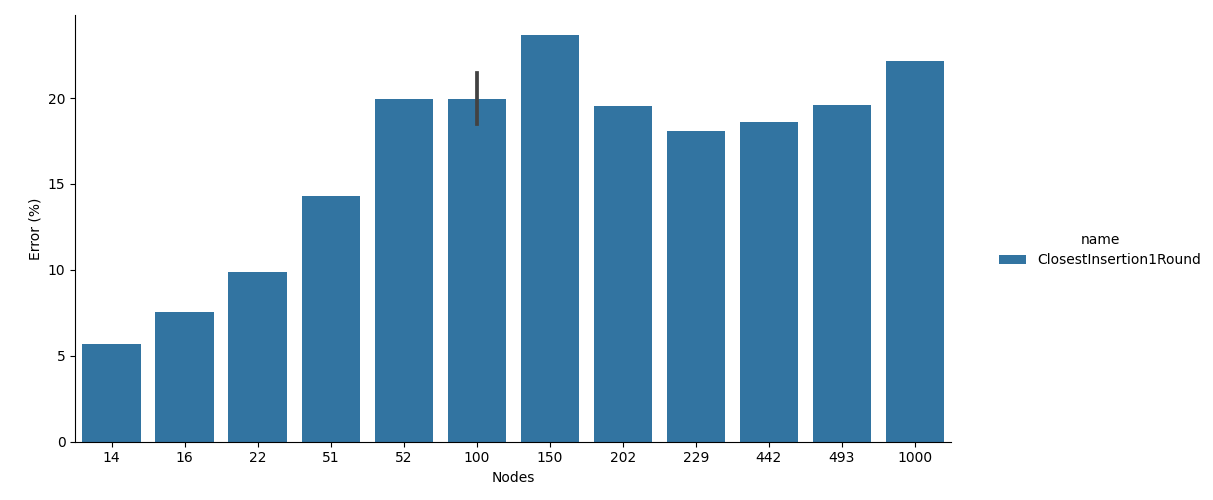
\includegraphics[width=0.9\textwidth]{./images/ClosestInsertion1Round__approximation_error_.png}

    \caption{Errore introdotto da ClosestInsertion rispetto al numero di nodi.}
    \label{fig:closest-insertion-1-round-accuracy-error}
\end{figure}
